%=============================================================================
%\documentclass[11pt,twoside]{article}
\documentclass[11pt,a4paper,twoside,bibtotoc]{scrartcl}
%\documentclass[twoside,11pt]{article}
%\usepackage{jnm}
%=============================================================================
\usepackage{a4wide}
\usepackage{amsfonts}
\usepackage{amsmath}
\usepackage{theorem}
%\usepackage{jkmath}
\usepackage{subfigure}
\usepackage{natbib}
\usepackage{algorithm}
\usepackage{algorithmic}
\usepackage{graphicx}

\theoremstyle{plain}
\newtheorem{theorem}{Theorem}[section]
\newtheorem{corollary}[theorem]{Corollary}
\newtheorem{lemma}[theorem]{Lemma}
\newtheorem{proposition}[theorem]{Proposition}
\theoremstyle{definition}
\newtheorem{definition}[theorem]{Definition}
\newtheorem{example}[theorem]{Example}
\theoremstyle{remark}
\newtheorem{remark}[theorem]{Remark}
\newenvironment{proof}{{\bf Proof.}}{$\Box$}

\newcommand{\adj}{{\vdash \hspace*{-1.72mm} \dashv}}
\newcommand{\supp}{\:{\rm supp}}

\renewcommand{\topfraction}{1}
\renewcommand{\textfraction}{0}
\setcounter{totalnumber}{4}

%============================================================================

\newcommand{\N}{\ensuremath{\mathbb{N}}}
\newcommand{\NZ}{\ensuremath{\mathbb{N}_{0}}}
\newcommand{\Z}{\ensuremath{\mathbb{Z}}}
\newcommand{\Q}{\ensuremath{\mathbb{Q}}}
\newcommand{\R}{\ensuremath{\mathbb{R}}}
\newcommand{\Rp}{\ensuremath{\mathbb{R}^{+}}}
\newcommand{\Rn}{\ensuremath{\mathbb{R}^n}}
\newcommand{\Rnn}{\ensuremath{\mathbb{R}^{n \times n}}}
\newcommand{\C}{\ensuremath{\mathbb{C}}}
\newcommand{\Pol}{\ensuremath{\Pi}}

\newcommand{\norm}[1]{\ensuremath{\left\|#1\right\|}}
\newcommand{\abs}[1]{\ensuremath{\left\vert#1\right\vert}}
\newcommand{\set}[1]{\ensuremath{\left\{#1\right\rbrace}}
\newcommand{\pset}[3]{\ensuremath{\left\{#1\ \left#2\ #3\right.\right\rbrace}}
\newcommand{\veps}{\ensuremath{\varepsilon}}
\newcommand{\vtheta}{\ensuremath{\vartheta}}
\newcommand{\vphi}{\ensuremath{\varphi}}
\newcommand{\towards}{\ensuremath{\longrightarrow}}

\newcommand{\twosphere}{\ensuremath{\mathbb{S}^2}}
\newcommand{\Ln}[2]{\ensuremath{\text{\rm{L}}^{#1}\left(#2\right)}}
\newcommand{\interv}[4]{\ensuremath{\left#1\left.#2,#3\right#4\right.}}
\newcommand{\fun}[2]{\ensuremath{#1{\hspace{-0.4ex}}\left(#2\right)}}
\newcommand{\paren}[1]{\ensuremath{\left(#1\right)}}
\newcommand{\encl}[3]{\ensuremath{\left#1#2\right#3}}
\newcommand{\bigo}[1]{\ensuremath{\mathcal{O}\paren{#1}}}
\newcommand{\smallo}[1]{\ensuremath{\mathcal{o}\paren{#1}}}
\newcommand{\jkSpacer}{\ensuremath{{}^{}}}
\newcommand{\scalarproduct}[2]{\ensuremath{\left<#1,#2\right>}}
\newcommand{\mb}[1]{\mathbf{#1}}
\newcommand{\V}[1]{\mb{#1}}
\newcommand{\transp}{\text{\rm{T}}}
\newcommand{\h}{\text{\rm{H}}}
\newcommand{\dx}{\text{\rm{d}}}
\renewcommand{\Re}{\text{\rm{Re}}}
\renewcommand{\Im}{\text{\rm{Im}}}
\newcommand{\e}{\mbox{\rm{e}}}
\newcommand{\im}{\mbox{\scriptsize\rm{i}}}
\newcommand{\diag}{\text{\rm{diag}}}
\def\invisible#1{\textcolor{white}{#1}}
\newcommand{\ceil}[1]{\encl{\lceil}{#1}{\rceil}}
\newcommand{\floor}[1]{\encl{\lfloor}{#1}{\rfloor}}

%============================================================================

\numberwithin{equation}{section}
\numberwithin{table}{section}
\numberwithin{figure}{section}

%\newlength{\temp}
%\setcounter{totalnumber}{10}
%\setcounter{topnumber}{10}

%============================================================================

\title{
%{\rm\normalsize Short Note}\\
Fast Summation on the sphere}

\date{\today}

\author{
Jens Keiner\thanks{keiner@math.uni-luebeck.de, University of
  L\"ubeck, Institute of Mathematics, D--23560 L\"ubeck} \and
Stefan Kunis\thanks{kunis@math.uni-luebeck.de, University of
  L\"ubeck, Institute of Mathematics, D--23560 L\"ubeck} \and
Daniel Potts\thanks{potts@math.uni-luebeck.de, University of
  L\"ubeck, Institute of Mathematics, D--23560 L\"ubeck} 
}

%=============================================================================
\begin{document}
\maketitle

\begin{abstract}
\medskip

%\noindent
%2000 {\it Mathematics Subject Classification}. 65F10, 65F15, 65T40.

\noindent
{\it Key words and phrases}.  
\end{abstract}

%-----------------------------------------------------------------------------
\section{Introduction}
\label{sect:1}
Radial basis functions are a powerful tool in many areas of multi-dimensional 
approximation and interpolation.
In radial basis function methods one approximates functions from $\R^3
\rightarrow \R$ by linear combinations of translates of a single radial 
symmetric function $\phi:\R^3 \rightarrow \R, \, \phi(x)=\phi(\|x\|_2)$.
The spherical counterpart are the \emph{zonal} functions which depent solely
on the geodesic distance of two points on the sphere $\twosphere:=\{
\V{\xi}: \|\V{\xi}\|_2=1\} \subset \R^3$ and the notion of the former
translation is replaced by the usual inner product.
More formally, let $K \in \Ln{2}{\interv{[}{-1}{1}{]}}$ and define for fixed
$\V{\eta} \in \twosphere$ the $\V{\eta}$-zonal function 
\[
  \fun{K}{\V{\eta} \: \cdot}: \twosphere \rightarrow \R,\ \V{\xi} \mapsto
  \fun{K}{\V{\eta} \cdot \V{\xi}}\,.% \qquad \V{\xi} \in \twosphere.
\]
Of course, every radial function corresponds to a zonal function by means of
\[
  \fun{K}{\V{\eta} \cdot \V{\xi}} = \phi\left(\sqrt{2-2\V{\eta} \cdot
  \V{\xi}}\right)\,.
\]

\section{Prerequisites}
\label{sect:2}
The Legendre polynomials $P_k : \interv{[}{-1}{1}{]} \rightarrow \R$, $k \in
\N_{0}$ as classical orthogonal polynomials are given by their corresponding
\emph{Rodrigues formula}
\[
\fun{P_k}{x} := \frac{1}{2^k k!} \frac{\dx^k}{\dx x^k} \paren{x^2-1}^k.
\]
One verifies $\fun{P_{k}}{\pm1} = \paren{\pm1}^{k}$, $\left|\fun{P_{k}}{\cos\vartheta}\right|
\le \sqrt{\frac{2}{\pi k \sin\vartheta}}$ for $\vartheta \in (0,\pi)$, $k \ge 1$, 
and $\max_{x \in \interv{[}{-1}{1}{]}} \abs{\fun{P_{k}}{x}} = 1$, 
\cite[pp. 47]{niuv}.
Furthermore, two recurrence relations are given by
\begin{equation}\label{three1}
\paren{k+1}\fun{P_{k+1}}{x} = \paren{2k+1}x\fun{P_{k}}{x} - k\fun{P_{k-1}}{x}
\end{equation}
and
\begin{equation}\label{three2}
\paren{2k+1} \fun{P_{k}}{x} = \fun{P_{k+1}'}{x} - \fun{P_{k-1}'}{x}.
\end{equation}

Let the space of real-valued continuous functions on the sphere be decomposed
into the direct sum of spaces of spherical harmonics, i.e.,
$C(\twosphere)=\bigoplus_{k=0}^{\infty} \mathcal{H}_k$ and let
$\set{Y_{k}^n}_{k \in \NZ; n=-k,\ldots,k}$ denote the 
standard orthonormal basis of spherical harmonics given by
\[
  \fun{Y_{k}^n}{\V{\xi}} = \fun{Y_{k}^n}{\vartheta,\varphi} = 
  \sqrt{\frac{2k+1}{4\pi}} 
  \fun{P_{k}^{|n|}}{\cos\vartheta} \e^{\im n \varphi}.
\]
The orthogonal expansion of the zonal function $\fun{K}{\V{\eta} \: \cdot}$
is given by,
\begin{equation}
  \label{equation:kernelExpansion}
  \fun{K}{\V{\eta} \cdot \V{\xi}} = \sum_{k = 0}^{\infty} \sum_{n=-k}^k
  \fun{K^{\wedge}}{k}\overline{\fun{Y_{k}^n}{\V{\eta}}} \fun{Y_{k}^n}{\V{\xi}}
  = \sum_{k = 0}^{\infty} \frac{2k+1}{4\pi} \fun{K^{\wedge}}{k}
  \fun{P_{k}}{\V{\eta} \cdot \V{\xi}},
\end{equation}
where we use the addition theorem
\[
\sum_{n=-k}^{k} \fun{Y_{k}^n}{\V{\xi}} \overline{\fun{Y_{k}^n}{\V{\eta}}} =
    \frac{2k+1}{4\pi}\fun{P_k}{\V{\eta} \cdot \V{\xi}}
\]
and the \emph{Legendre transform}, i.e. the \emph{symbol} of $K$, is given
for $k \in \NZ$ by
\begin{equation}
  \label{equation:legtrafo}
  \fun{K^{\wedge}}{k} := 2 \pi \int_{-1}^{1} \fun{K}{x} \fun{P_{k}}{x} \dx 
  x\,.
\end{equation}

Note, that the first representation in \eqref{equation:kernelExpansion} allows
the construction of fast algorithms, which is due to the separation of the
knots $\V{\eta}$ and $\V{\xi}$.
Using the second representation of Equation \eqref{equation:kernelExpansion} in
conjunction with \eqref{equation:legtrafo} and the recurrence relations
\eqref{three1} and \eqref{three2} yields efficient ways to precompute the
needed coefficients $\fun{K^{\wedge}}{k}$.

Furthermore, we use the following convolution lemma which yields a possibility to trade
localisation of a zonal function in spatial domain against the decay of its
symbol.
More formally, we state
\begin{lemma} {\bf Normalisierung!!}
  Let $Q,P\in \Ln{2}{\interv{[}{-1}{1}{]}}$ and
  \[
  \fun{K}{\V{\eta} \cdot \V{\xi}} := \fun{\left(Q * P\right)}{\V{\eta} \cdot
    \V{\xi}},
  \]
  where
  \[
    \fun{\left(Q * P\right)}{\V{\eta} \cdot \V{\xi}}:= 
    \int_{\twosphere} \fun{Q}{\V{\eta} \cdot \V{\nu}}
    \fun{P}{\V{\nu} \cdot \V{\xi}} \dx \omega\left(\nu\right)
  \]
  is the \emph{spherical convolution} of $Q$ and $P$. Then the symbol 
  $\fun{K^{\wedge}}{k}$ is given by 
  $\fun{K^{\wedge}}{k} = \fun{Q^{\wedge}}{k} \fun{P^{\wedge}}{k}$.
  Furthermore, for compactly supported functions $\supp\; Q = \supp\; P =
  \interv{[}{h}{1}{]}$, $h>0$, we conclude $\supp\; K =
  \interv{[}{2h^2-1}{1}{]}$.
\end{lemma}

\section{Fast Summation}
Given a set of arbitrary \emph{source nodes} $\mathcal{Y} :=
  \pset{\V{\eta}_{l} \in \twosphere}{|}{l = 0,\ldots,L-1}$ and a vector of
  real coefficients $\V{b}:=(b_{l})_{l=0}^{L-1}$, our goal consists in the fast
evaluation of sums 
\begin{equation}
  \label{Applications:KernelSum}
  \fun{f}{\xi} := \sum_{l = 0}^{L-1} b_{l} \fun{K}{\V{\eta}_{l} \cdot \V{\xi}}
\end{equation}
on a set of arbitrary \emph{target nodes} $\mathcal{X} := \pset{\V{\xi}_{d}
  \in \twosphere}{|}{d=0,\ldots,D-1}$.

Given an explicit expression, the zonal function $\fun{K}{\V{\eta} \: \cdot}$ 
can be evaluated easily or all the values 
$\fun{K}{\V{\eta}_{l} \cdot \V{\xi}_{d}}$ can be stored in
advance. The naive approach evaluating \eqref{Applications:KernelSum} leads to
an $\bigo{L\:D}$ algorithm. 
For large $L$ and $D$ the computational effort becomes quickly unaffordable.
The \emph{panel clustering} method introduced in \cite{FrGlSch98} reduces the
computational effort to evaluate \eqref{Applications:KernelSum} based on the
traditional method of dividing the evaluation into near- and far-field.
For every zonal function $\fun{K}{\V{\eta}_l \: \cdot}$, the near-field contribution
is calculated exactly whereas the contribution of the far-field may be
approximated coarsly.
% due to the supposed rapid decay of $\fun{K}{\V{\eta} \:\cdot}$. 

We propose to simply truncate the series \eqref{Basics:Kernel} at degree 
$M \in \NZ$, i.e.
\begin{equation}
  \label{Applications:TruncatedSeries}
  \fun{K}{\V{\eta}_{l} \cdot \V{\xi}} \approx \fun{K_{M}}{\V{\eta}_{l} \cdot
  \V{\xi}} := \sum_{k=0}^{M} \sum_{n=-k}^k \fun{K^{\wedge}}{k}
  \fun{Y_{k}^n}{\V{\xi}} \overline{\fun{Y_{k}^n}{\V{\eta}_{l}}}.
\end{equation}

Substituting \eqref{Applications:TruncatedSeries} into
\eqref{Applications:KernelSum} and interchanging the order of summation we
finally obtain the approximation
\[
  \fun{f_{M}}{\xi_{d}} := \sum_{k=0}^{M} \sum_{n=-k}^k \fun{K^{\wedge}}{k}
  \paren{\sum_{l = 0}^{L-1} b_{l} \overline{\fun{Y_{k}^n}{\V{\eta}_{l}}}}
  \fun{Y_{k}^n}{\V{\xi}_{d}}.
\]

The expression in the inner brackets can be computed by an adjoint Nonuniform
Fast Spherical Fourier Transform (adjoint NFSFT) in 
$\mathcal{O}(L + M^2 \log^2 M)$
arithmetic operations, see \cite{xxx} and the forthcoming paper \cite{xxx} for
details.
This is followed by $(M+1)^2$ multiplications with the symbol
$\fun{K^{\wedge}}{k}$, and completed by a NFSFT to compute the outer sum in
$\mathcal{O}(D + M^2 \log^2 M)$ arithmetic operations.
In Section \ref{Basics:SphericalKernels}, we will decompose the error and show
that the degree $M$ depends only on the desired accuracy of our algorithm and
on the particular zonal function $\fun{K}{\V{\eta} \: \cdot}$, but not on the
numbers $L$ and $D$.
Thus, the overall arithmetic complexity of our algorithm is $\mathcal{O}(L +
D)$, in particular this performance does not depend on the distribution of the
nodes $\V{\xi}_{d}$ and $\V{\eta}_{l}$.

\begin{remark}
  NFSFT ist auch nur approximativ. Referenzen zu Driscoll, Healy, usw..... 
  (Aufbau des Algorithmus)
\end{remark}

\begin{remark}
In matrix-vector notation the proposed approach, a particular rank $(M+1)^2$
approximation, read as
\[
  \V{f} = \V{Y_{\mathcal{X}}} \: \V{\hat W} \:
  \V{Y_{\mathcal{Y}}}^{\adj} \: \V{b}
\]
with
\begin{align}
  \nonumber
  \V{f} & := \paren{\fun{f}{\V{\xi}_{d}}}_{d=0}^{D-1} \in \R^D,
  \\ \nonumber
  \V{Y_{\mathcal{X}}} & := \paren{\fun{Y_k^n}{\V{\xi}_{d}}}_{d=0,\ldots,D-1;
  k=0,\ldots,M,\:n=-k,\ldots,k} \in \C^{D \times
  \paren{M+1}^2}, \\ \nonumber
  \V{\hat W} & := \fun{\diag}{\V{\hat w}},\ \V{\hat w} := \paren{\hat
  w_{k}^{n}}_{k=0,\ldots,M,\:n=-k,\ldots,k} \in \R^{(M+1)^2},\ \hat w_{k}^n :=
  \fun{K^{\wedge}}{k}, \\ \nonumber
  \V{Y_{\mathcal{Y}}} & := \paren{\fun{Y_k^n}{\V{\eta}_{l}}}_{l=0,\ldots,L-1;
  k=0,\ldots,M,\:n=-k,\ldots,k} \in \C^{L \times \paren{M+1}^2}.
\end{align}

Replacing the NFSFT by its slow version, which takes $\mathcal{O}(L M^2)$ and
$\mathcal{O}(D M^2)$ arithmetic operations, respectively, yields an
$\mathcal{O}(L+D)$ algorithm, too.
\end{remark}

In summary, we propose the following algorithm.
\begin{algorithm}[h]
  \caption{Fast Summation}
  \label{Applications:Algorithm:FastSummation}    
  \begin{algorithmic}
    \STATE  Input:  $L \in \N$, $\paren{b_{l}}_{l=0}^{L-1}$, $\paren{\V{\eta}_{l}}_{l=0}^{L-1}$, 
                    $D \in \N$, $\paren{\V{\xi}_{d}}_{d=0}^{D-1}$, $M \in \NZ, \paren{\fun{K^{\wedge}}{k}}_{k=0}^M$
    \STATE
    \STATE Compute $\V{\tilde{b}} := \V{Y_{\mathcal{Y}}}^{\adj} \: \V{b}$ by an
                    adjoint NFSFT 
    \FOR {$k=0,\ldots,M$} 
      \FOR {$n=-k,\ldots,k$} 
        \STATE Set $a_{k}^n := \tilde{b}_{k}^n \: \fun{K^{\wedge}}{k}$
      \ENDFOR
    \ENDFOR
    \STATE Compute $\V{f} := \V{Y_{\mathcal{X}}} \: \V{a}$ by a NFSFT
    \STATE
    \STATE Output: $\paren{\fun{f}{\V{\xi}_{d}}}_{d=0}^{D-1}$ (an approximation to 
      $\paren{\fun{f}{\V{\xi}_{d}}}_{d=0}^{D-1}$)
    \STATE
    \STATE Complexity: $\mathcal{O}\left(M^2 \log^2M + L + D\right)$  
\end{algorithmic}
\end{algorithm}


%--------------------------------------------------------------------------
\section{Error estimates and examples}\label{Basics:SphericalKernels}
%--------------------------------------------------------------------------
\begin{lemma}\label{lemma:error}
  The proposed approximation obeys the uniform error estimate
  \begin{equation*}
    \left\|\V{f} - \V{f}_{M}\right\|_{\infty} \le \left\|\V{b}\right\|_1 \sum_{k>M}
    \frac{2k+1}{4\pi} \abs{\fun{K^{\wedge}}{k}}.
  \end{equation*}
%  Moreover, if we assume random uniformly distributed source and target nodes, 
%  then we obtain the asymptotic bound
%  \begin{equation*}
%    \left\|\V{f} - \V{f}_{M}\right\|_{\infty} \le \left\|\V{b}\right\|_1 
%    \frac{2 \fun{\Gamma^2}{\frac{3}{4}}}{4\pi^2} \left( 2 \sum_{k>M} 
%    \sqrt{k} \abs{\fun{K^{\wedge}}{k}} + \sum_{k>M} \frac{1}{\sqrt{k}} 
%    \abs{\fun{K^{\wedge}}{k}}\right).
%  \end{equation*}
\end{lemma}
\begin{proof}
  We obtain immediately
  \begin{align*}
    \left\|\V{f} - \V{f}_{M}\right\|_{\infty} 
    & = \max_{\V{\xi} \in \mathcal{X}} 
        \left|\sum_{l=0}^{L-1} b_{l} \sum_{k>M} \frac{2k+1}{4\pi} \fun{K^{\wedge}}{k} 
        \fun{P_{k}}{\V{\eta}_{l} \cdot \V{\xi}}\right| \\
    & \le \sum_{l=0}^{L-1} \left| b_{l} \right| \max_{\V{\xi} \in \mathcal{X}} \left| \sum_{k>M} 
          \frac{2k+1}{4\pi} \fun{K^{\wedge}}{k} \fun{P_{k}}{\V{\eta}_{l} \cdot \V{\xi}} \right| \\
    & \le \left\|\V{b}\right\|_1 \sum_{k>M} \frac{2k+1}{4\pi} \abs{\fun{K^{\wedge}}{k}},
  \end{align*}
  where, we have used $\left|\fun{P_{k}}{x}\right| \le 1$. 
%  If we now asume random uniformly 
%  distributed source and target nodes, we might replace this estimate in the asymptotic sense, i.e.
%  for $L,D \towards \infty$ by the expected value
%  \begin{equation*}
%    E_{k} := \int_{0}^{\pi} \fun{P_{k}}{\cos\vartheta} \fun{p}{\vartheta} \; \dx \vartheta,
%  \end{equation*}
%  where $\fun{p}{\vartheta} := \frac{\sin\vartheta}{2}$ is the probability for a source node 
%  $\V{\eta}$ and a target node $\V{\xi}$ to span the angle $\vartheta$. 
%  Now using the estimate
%  $\left|\fun{P_{k}}{\cos\vartheta}\right| \le \sqrt{\frac{2}{\pi k \sin\vartheta}}$ for 
%  $\vartheta \in \left(0, \pi\right)$ yields
%  \begin{equation*}
%    E_{k} 
%    \le \int_{0}^{\pi} 
%          \sqrt{\frac{2}{\pi k \sin\vartheta}} \frac{\sin\vartheta}{2} \; \dx \vartheta \\
%      = \int_{0}^{\pi} \sqrt{\frac{\sin\vartheta}{2 \pi k }} \; \dx \vartheta \\
%      = \frac{2 \fun{\Gamma^2}{\frac{3}{4}}}{\pi\sqrt{k}}.
%  \end{equation*}
%  We obtain finally
%  \begin{align*}
%    \left\|\V{f} - \V{f}_{M}\right\|_{\infty} 
%    & \le \left\|\V{b}\right\|_1 \frac{2 \fun{\Gamma^2}{\frac{3}{4}}}{\pi} \sum_{k>M} 
%    \frac{2k+1}{4\pi\sqrt{k}} \abs{\fun{K^{\wedge}}{k}}\\
%    & \le \left\|\V{b}\right\|_1 \frac{2 \fun{\Gamma^2}{\frac{3}{4}}}{4\pi^2} \left( 2 \sum_{k>M} 
%    \sqrt{k} \abs{\fun{K^{\wedge}}{k}} + \sum_{k>M} \frac{1}{\sqrt{k}} \abs{\fun{K^{\wedge}}{k}}\right)\\
%  \end{align*}
%  Now using the estimates
%  $\left|\fun{P_{k}}{\cos\vartheta}\right| \le \sqrt{\frac{2}{\pi k \sin\vartheta}}$ for 
%  $\vartheta \in \left[\arcsin \frac{2}{\pi k}, \pi - \arcsin \frac{2}{\pi k}\right]$ and 
%  $\left|\fun{P_{k}}{\cos\vartheta}\right| \le 1$ for $\vartheta \in \left[0, \arcsin 
%  \frac{2}{\pi k}\right)\cup \left( \pi-\arcsin\frac{2}{\pi k}, \pi\right]$ yields
%  \begin{align*}
%    E_{k} 
%    & \le 2\arcsin\frac{2}{\pi k} + 
%          \int_{\arcsin\frac{2}{\pi k}}^{\pi - \arcsin\frac{2}{\pi k}} 
%          \sqrt{\frac{2}{\pi k \sin\vartheta}} \frac{\sin\vartheta}{2} \; \dx \vartheta \\
%    &   = 2\arcsin\frac{2}{\pi k} +  \int_{\arcsin\frac{2}{\pi k}}^{\pi - \arcsin\frac{2}{\pi k}} 
%          \sqrt{\frac{\sin\vartheta}{2 \pi k }} \; \dx \vartheta \\
%    &   = 2\arcsin\frac{2}{\pi k} - \frac{4}{\sqrt{2\pi k}} \fun{E}{\frac{\arcsin\frac{2}{\pi k}}{2} - \frac{\pi}{4},2},
%  \end{align*}
%  and \fun{E}{\phi,j} is the elliptic integral of the second kind
%  \begin{equation*}
%    \fun{E}{\phi,j} := \int_{0}^{\phi} \sqrt{1-j^2\sin^2 \theta} \: \dx \theta.
%  \end{equation*}
%  We obtain finally
%  \begin{equation*}
%    \left\|\V{f} - \V{f}_{M}\right\|_{\infty} 
%    \le \left\|\V{b}\right\|_1 \left(2\sum_{k>M} \fun{\arcsin}{\frac{2}{\pi k}} \frac{2k+1}{4\pi} \abs{\fun{K^{\wedge}}{k}} - 
%    \frac{4}{\sqrt{2\pi}} \sum_{k>M} \fun{E}{\frac{\arcsin\frac{2}{\pi k}}{2} - \frac{\pi}{4},2} \frac{2k+1}{4\pi\sqrt{k}} 
%    \abs{\fun{K^{\wedge}}{k}}\right),
%  \end{equation*}
\end{proof}

\subsection{Poisson and Singularity kernel}
\begin{definition}
  Let $h \in \interv{(}{0}{1}{)}$, then the
  \begin{enumerate}
  \item \emph{Poisson kernel}
    $Q_{h}:\interv{[}{-1}{1}{]} \rightarrow \R$ is given by
    \[
    \fun{Q_{h}}{x} := \frac{1}{4\pi} \frac{1-h^2}{\paren{1-2hx+h^2}^{3/2}}\,.
    \]
  \item and the \emph{singularity kernel}
    $S_{h}:\interv{[}{-1}{1}{]} \rightarrow \R$ is given by
    \[
    \fun{S_{h}}{x} := \frac{1}{2\pi} \frac{1}{\paren{1-2hx+h^2}^{1/2}},
    \]
  \end{enumerate}
\end{definition}

We refer to Figure \ref{Basics:Figure:PoissonSingularityKernel} for a visual
impression and mention that the parameter $h$ allows for controlling the
concentration of $\fun{Q_{h}}{\V{\eta} \: \cdot}$ and $\fun{S_{h}}{\V{\eta} \:
  \cdot}$ around $\eta \in \twosphere$, respectively.
The Poisson kernel is a positive function and normalized with
$\|\fun{Q_{h}}{\V{\eta} \: \cdot}\|_{\Ln{1}{\twosphere}}$.
Further properties with respect to localization and smoothness are derived
in \cite[pp. 112]{frgesc}.

\begin{figure}[tb]
  \centering
  \subfigure[$h=0.5,0.7,0.8$]
  {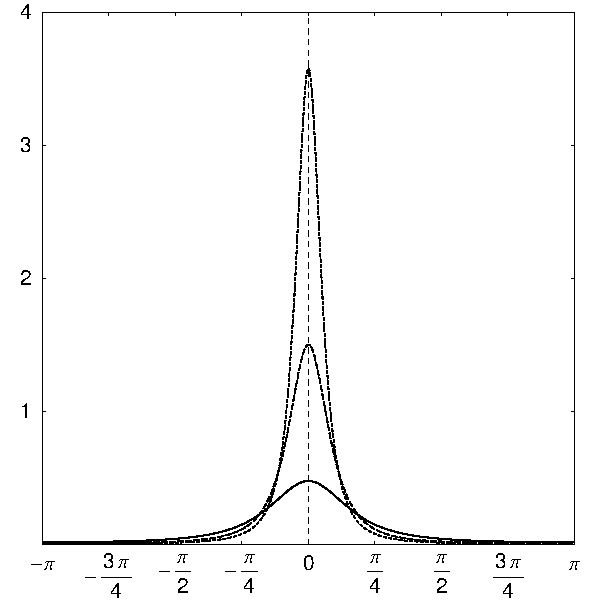
\includegraphics[width=0.45\textwidth]{images/poisson}}\hfill
  \subfigure[$h=0.8,0.9,0.955$]
  {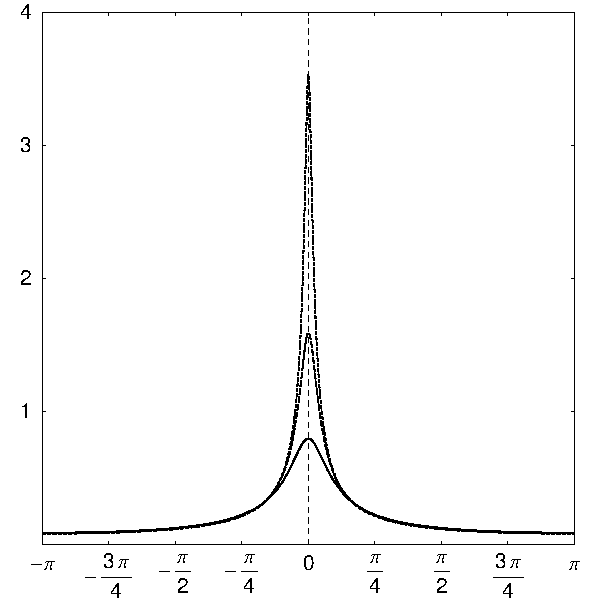
\includegraphics[width=0.45\textwidth]{images/singularity}}
  \caption{The kernels $\fun{Q_{h}}{\cos\vartheta}$ and $\fun{S_{h}}{\cos\vartheta}$
  for different values of $h$.}
  \label{Basics:Figure:PoissonSingularityKernel}
\end{figure}

For both kernels the symbol is explicitely known, such that we easily state
the following lemma.
\begin{lemma}
 Using these kernels within our summation algorithm yields an relative error
 of
 \begin{enumerate}
   \item
     \begin{equation}
       \label{error:poisson}
       \frac{\left\|f - f_{M}\right\|_{\infty}}{\left\|\V{b}\right\|_1} \le
       \frac{h^{M+1}}{4\pi} \left(\frac{2M+1}{1-h}+\frac{2}{\left(1-h\right)^2}\right)
     \end{equation}
     for the Poisson kernel and
     \item 
       \begin{equation}
         \label{error:singular}
         \frac{\left\|f - f_{M}\right\|_{\infty}}{\left\|\V{b}\right\|_1} \le
         \frac{h^{M+1}}{4\pi} \left(\frac{2M+1}{2\left(1-h\right)}+
           \frac{4M}{\left(1-h\right)^2}+ \frac{4}{\left(1-h\right)^3}\right),
       \end{equation}
       for the singularity kernel, respectively.
 \end{enumerate}
\end{lemma}
\begin{proof}
The symbols are given by $\fun{Q_{h}^{\wedge}}{k}=h^k$ and
$\fun{S_{h}^{\wedge}}{k}=\frac{2}{2k+1}h^k$, respectively.
Using Lemma \ref{lemma:error} yields the assertions.
\end{proof}
  
Simply put, our scheme (almost) achieves accuracy $\epsilon$ for $M \ge \log\epsilon \,
/ \, \log h$.

\subsection{Locally supported kernel}
\begin{definition}
  Let $h \in \interv{(}{0}{1}{)}$ and $\lambda,\mu \in \NZ$.
  \begin{enumerate}
  \item A locally supported zonal function
    $L_{h,\lambda}:\interv{[}{-1}{1}{]} \rightarrow \R$, considered in
    \cite{Sc97}, is defined by
    \[
    \fun{L_{h,\lambda}}{x} := 
    \left\{\begin{array}{l@{\quad \text{if} \quad}rcl} 
        0 & -1 &\le x \le& h, \\
        \frac{\lambda+1}{2\pi(1-h)^{\lambda+1}}\paren{x-h}^{\lambda} &  h & <  x \le& 1,
      \end{array}\right.
    \]
  \item Furthermore, we define by iterated spherical convolution
    \[
    L_{h,\lambda,\mu} = L_{h,\lambda,\mu-1} * L_{h,\lambda},
    \]
    where $L_{h,\lambda,1}=L_{h,\lambda}$.
  \end{enumerate}
\end{definition}

Figure \ref{Basics:Figure:LKernel} shows the function $L_{h,\lambda}$ for
different values $h$ and $\lambda$.
\begin{figure}[tb]
  \centering
  \subfigure[$\lambda=1.0$]
  {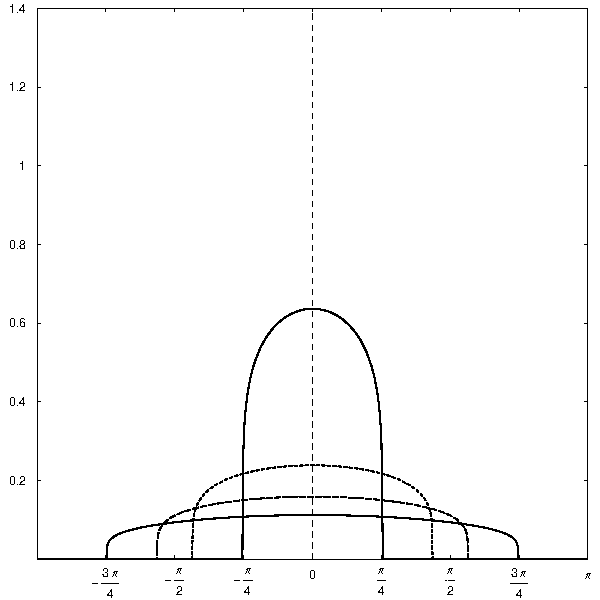
\includegraphics[width=0.45\textwidth]{images/locsup1}}\hfill
  \subfigure[$\lambda=2.0$]
  {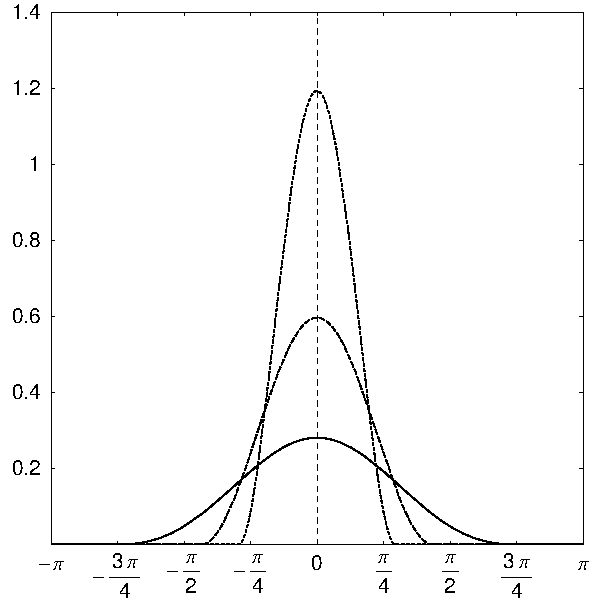
\includegraphics[width=0.45\textwidth]{images/locsup2}}
  \caption{The kernel $L_{h,\lambda}$ for $h = -0.7, 0.2, 0.7$ and different values of $\lambda$.}
  \label{Basics:Figure:LKernel}
\end{figure}
While the parameter $h$ again steers the localisation in spatial domain, the
parameter $\lambda$ correponds to the smoothness in spatial domain.
The iterated kernel $L_{h,\lambda,\mu}$ trades localisation in spatial domain
for localisation in frequency domain by increasing $\mu$.
More formally, we have the following lemma.

\begin{lemma}
  We collect the following facts about the locally supported kernel.
  \begin{enumerate}
  \item The symbol $\fun{L_{h,\lambda}^{\wedge}}{k}$ can be computed recursively by
    \[
    \fun{L_{h,\lambda}^{\wedge}}{k+1} = \frac{\paren{2k+1} h}{k+\lambda+2}
    \fun{L_{h,\lambda}^{\wedge}}{k}   - \frac{k-\lambda-1}{k+\lambda+2}
    \fun{L_{h,\lambda}^{\wedge}}{k-1}
    \]
    for $k\in \N$, $\fun{L_{h,\lambda}^{\wedge}}{0} = 1$, and
    $\fun{L_{h,\lambda}^{\wedge}}{1} = \frac{\lambda + 1 + h}{\lambda+2}$.
  \item We obtain for fixed $\lambda \in \NZ$ the decay rate
    \[
    \left|\fun{L_{h,\lambda}^{\wedge}}{k}\right| \le C_{\lambda}
    \left(1-h\right)^{-\lambda-\frac{5}{4}} k^{-\lambda-\frac{3}{2}}.
    \]
  \item Thus, the relative error of our summation algorithm with this kernel
  is bounded for fixed $\lambda \in \N$ by
  \begin{equation}
    \label{error:Lh}
    \frac{\left\|f - f_{M}\right\|_{\infty}}{\left\|\V{b}\right\|_1} \le
    \tilde C_{\lambda} \left(1-h\right)^{-\lambda-\frac{5}{4}} M^{\frac{1}{2}-\lambda}.
  \end{equation}
  \end{enumerate}
\end{lemma}
\begin{proof}
  \begin{enumerate}
  \item We apply \eqref{three1} and \eqref{three2}.
  \item For $\lambda=0$ holds
    \[
    \left|\fun{L_{h,0}^{\wedge}}{k}\right| = \frac{1}{1-h}
    \left|\int_{h}^{1} \fun{P_{k}}{x} \dx x\right| \le
    \frac{\sqrt{2}}{\left(2k+1\right)\left(1-h\right)\sqrt{\pi}\sqrt[4]{1-h^2}}
    \left(\frac{1}{\sqrt{k-1}}+\frac{1}{\sqrt{k+1}}\right)\,.
    \]
    Applying \eqref{three2}, we obtain furthermore
    \begin{eqnarray*}
      \left|\fun{L_{h,\lambda}^{\wedge}}{k}\right| &\le&
      \frac{\lambda+1}{\lambda\left(1-h\right)\left(2k+1\right)}
      \left|\fun{L_{h,\lambda-1}^{\wedge}}{k-1}-
        \fun{L_{h,\lambda-1}^{\wedge}}{k+1}\right|\\ &\le&
      \frac{\lambda+1}{\lambda\left(1-h\right)\left(k+\frac{1}{2}\right)}
      \max\limits_{k-1\le k'\le k+1}
      \left|\fun{L_{h,\lambda-1}^{\wedge}}{k'}\right|
    \end{eqnarray*}
    Iterate this argument until $\lambda=0$ yields the assertion.
  \item We combine 2. with Lemma \ref{lemma:error}. 
  \end{enumerate}
\end{proof}

Simply put, our scheme achieves accuracy of order $\epsilon$ for $M \ge
(1-h)\sqrt[\lambda]{\epsilon}$.

\subsection{Gaussian kernel}
\begin{definition}
  For $\sigma>0$, the \emph{Gaussian kernel}
  $G_{\sigma}:\interv{[}{-1}{1}{]} \rightarrow \R$ is given by
  \begin{equation}
    \label{GaussKernel}
    \nonumber
    \fun{G_{\sigma}}{x} := \e^{2\sigma x-2\sigma}\,.
  \end{equation}
\end{definition}

Figure \ref{Basics:Figure:GKernel} shows the function $G_{\sigma}$ for
different values $\sigma$.
\begin{figure}[tb]
  \centering
  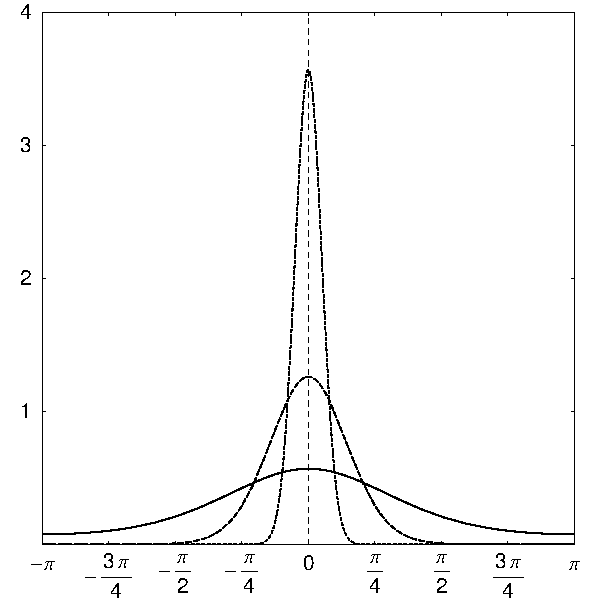
\includegraphics[width=0.7\textwidth]{images/gaussian}
  \caption{The Gaussian-kernel $G_{\sigma}$ for $\sigma = 2,10,80$.}
  \label{Basics:Figure:GKernel}
\end{figure}

\begin{lemma}
  Again, we collect some useful facts about kernel.
  \begin{enumerate}
  \item The symbol $\fun{G_{\sigma}^{\wedge}}{k}$ can be computed by a
    recurrence relation
    \[
    \fun{G_{\sigma}^{\wedge}}{k+1} = 
    \fun{G_{\sigma}^{\wedge}}{k-1}   - \frac{2k+1}{2\sigma}
    \fun{G_{\sigma}^{\wedge}}{k}
    \]
    for $k\in \N$, $\fun{G_{\sigma}^{\wedge}}{0} = 4 \pi \sigma^{-1}
    \e^{-2\sigma} \sinh \sigma \cosh \sigma$, and
    $\fun{G_{\sigma}^{\wedge}}{1} = \pi \sigma^{-2} \e^{-2\sigma} (2 \sigma
    \cosh 2 \sigma + \sinh \sigma )$.
  \item A 'closed' form of the symbol is given by
    \[
    \fun{G_{\sigma}^{\wedge}}{k} = 2 \sigma^{-\frac{1}{2}} \e^{-2\sigma}
    \pi^{\frac{3}{2}} I_{k+\frac{1}{2}}\left(2\sigma\right)
    \]
    where $I_{k+\frac{1}{2}}$ denotes the modified Bessel function of first kind.
    Furthermore, $\fun{G_{\sigma}^{\wedge}}{k} \ge 0$.
  \item Thus, the relative error of our summation algorithm with this kernel
  is bounded by
  \begin{equation}
    \label{error:G}
    \frac{\left\|f - f_{M}\right\|_{\infty}}{\left\|\V{b}\right\|_1} \le
    .
  \end{equation} 
\end{enumerate}
\end{lemma}
\begin{proof}
  \begin{enumerate}
  \item The relation \eqref{three2} and integration by parts yields the
  assertion.
  \item The solution of the difference equation in 1. is given by the modified
  Bessel function of first kind, cf. \cite{}.
  The nonnegativity follows readily from the fact that the Gaussian is a
  positive definite function, cf. \cite{}.
  \item Using 2. and
  \begin{eqnarray*}
    \sum_{k>M} \frac{2k+1}{4\pi} \abs{\fun{G_{\sigma}^{\wedge}}{k}}
    &=&
    \sum_{k>M} \frac{\e^{-2\sigma}
    \left(k+\frac{1}{2}\right)\sigma^k}{\fun{\Gamma}{k+1}} \int_{-1}^{1}
    \e^{2\sigma x} \left(1-x^2\right)^k \dx x\\
    &\le&
    \sum_{k>M} \frac{\left(k+\frac{1}{2}\right)\sigma^k}{\fun{\Gamma}{k+1}}
    \int_{-1}^{1} \left(1-x^2\right)^k \dx x\\
    &=&
    \sum_{k>M} \frac{\sqrt{\pi}\sigma^k}{\fun{\Gamma}{k+\frac{1}{2}}}\\
    &=&
    \frac{\sqrt{\pi\sigma}\e^{\sigma}}{\fun{\Gamma}{M+\frac{1}{2}}} 
    \int_{0}^{\sigma} t^{M-\frac{1}{2}} \e^{-t} \dx t\\
    &\le&
    \frac{\sqrt{\pi\sigma}\e^{\sigma} \sigma^{M+\frac{1}{2}}}{\fun{\Gamma}{M
    +\frac{1}{2}}}
  \end{eqnarray*}
  yields the assertion.
\end{enumerate}

\begin{corollary}
 Matrix norms ...
\end{corollary}
\end{proof}

%--------------------------------------------------------------------------
\section{Numerical Examples}
%--------------------------------------------------------------------------

We present numerical examples in order to demonstrate the performance of
our approach. All algorithms were implemented in C and tested on an 
AMD Athlon\texttrademark XP 2700+ with 2GB main memory, SuSe-Linux 
(kernel 2.4.20-4GB-athlon, gcc 3.3) using double precision arithmetic. 
Moreover, we have used the libraries FFTW 3.0.1 \cite{fftw}, NFFT 2
\cite{kupo02C} and a custom NFSFT library that will be part of the next 
major release of the NFFT library. Throughout our experiments we have 
applied the NFFT package \cite{kupo02C} with precomputed Kaiser--Bessel 
functions and an oversampling factor $\rho=2$.

In our tests we have always chosen uniformely distributed pseudo-random 
source and target nodes 
$\paren{\vartheta,\varphi} \in [0,\pi] \times [-\pi,\pi]$ and 
coefficients $b_l$ from $\left[-\frac{1}{2},\frac{1}{2}\right]$.

We have considered the following kernels:

\begin{itemize}
  \item Poisson kernel $Q_{h}$,
  \item SIngularity kernel $S_{h}$,
  \item Locally supported kernel $L_{h,\lambda}$,
  \item Gaussian kernel $G_{\sigma}$.
\end{itemize}


First, we examine the systematic error due to our approximation 
\eqref{Applications:TruncatedSeries} and the use of the 
approximative NFSFT algorithm. Figure \ref{fig:error} presents 
the error
\[
  E_{\infty}:=
  \frac{\max\limits_{d=0,\ldots,D-1}\left|\fun{f}{\xi_{d}}-
  \fun{f_{M}}{\xi_{d}}\right|}{\sum\limits_{k=0}^N 
  |b_l|} \quad \approx \quad \|K_{\text{ERR}}\|_{\infty}
\]
for the mentioned kernels as a function of the parameter $M$.
These results confirm the error estimates \eqref{error:poisson},
\eqref{error:singular} and \eqref{error:Lh}.

\begin{figure}[tb]
  \centering
  \subfigure[The Poisson kernel $Q_{h}$ for $h = 0.8$.]
  {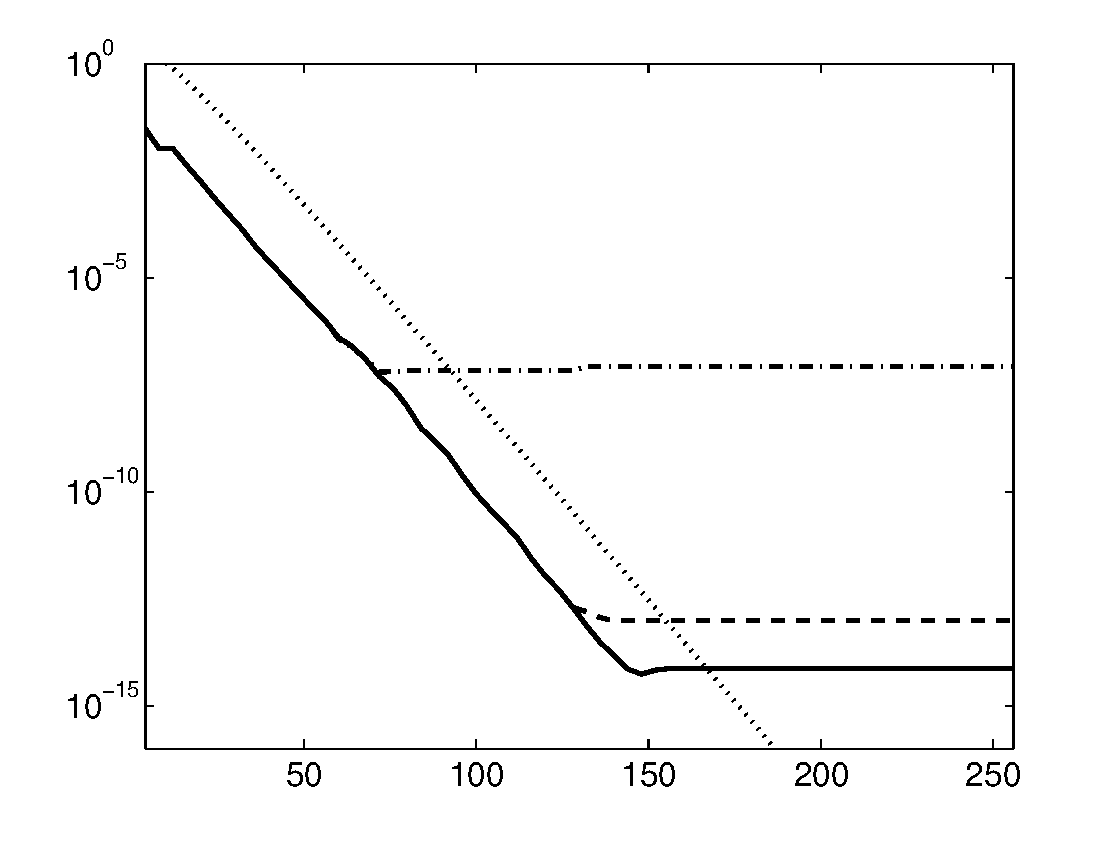
\includegraphics[width=0.45\textwidth]{images/poisson_test}}\hfill
  \subfigure[[The Singularity kernel $S_{h}$ for $h = 0.8$.]
  {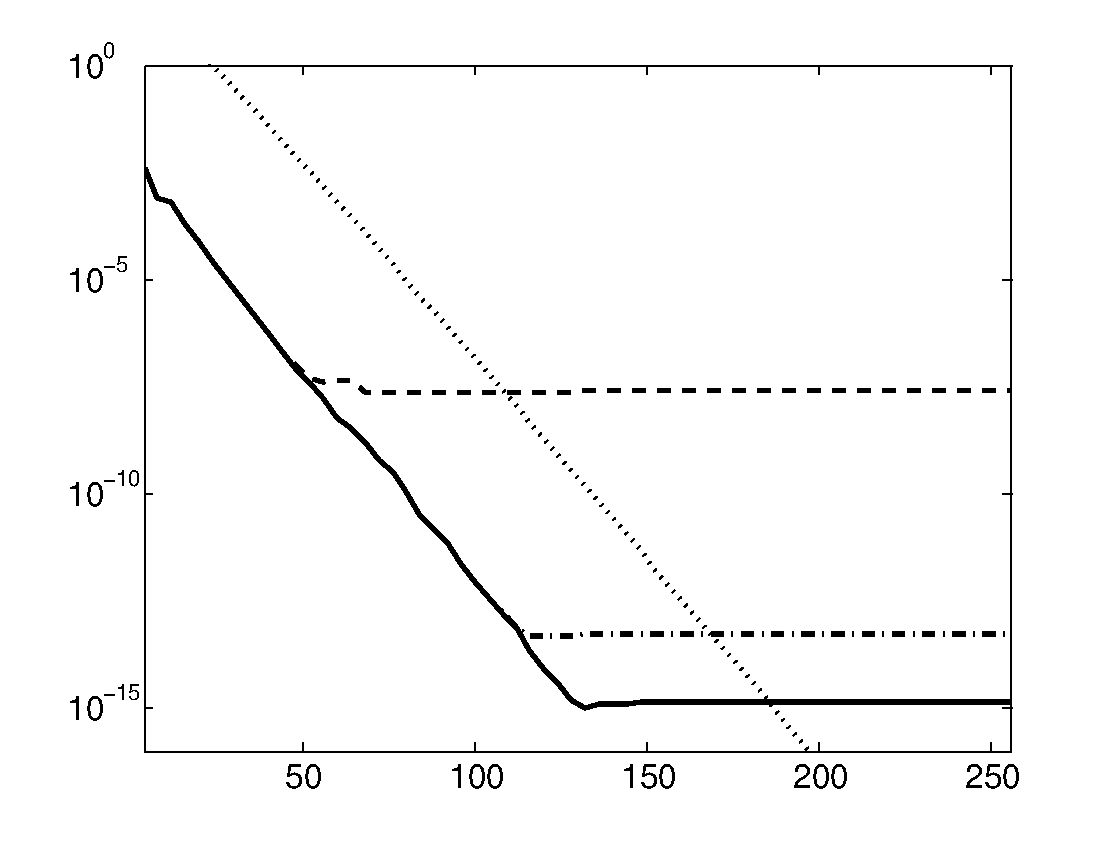
\includegraphics[width=0.45\textwidth]{images/singularity_test}}\\
  \subfigure[The locally supported kernel $L_{h,\lambda}$ for $h=0.3$, $\lambda = 7$. 
  The error estimate was fitted using $C_{\lambda} = 100$. For $C_{\lambda} = 50$ 
  the error estimate virtually coincides with the numerical result.]
  {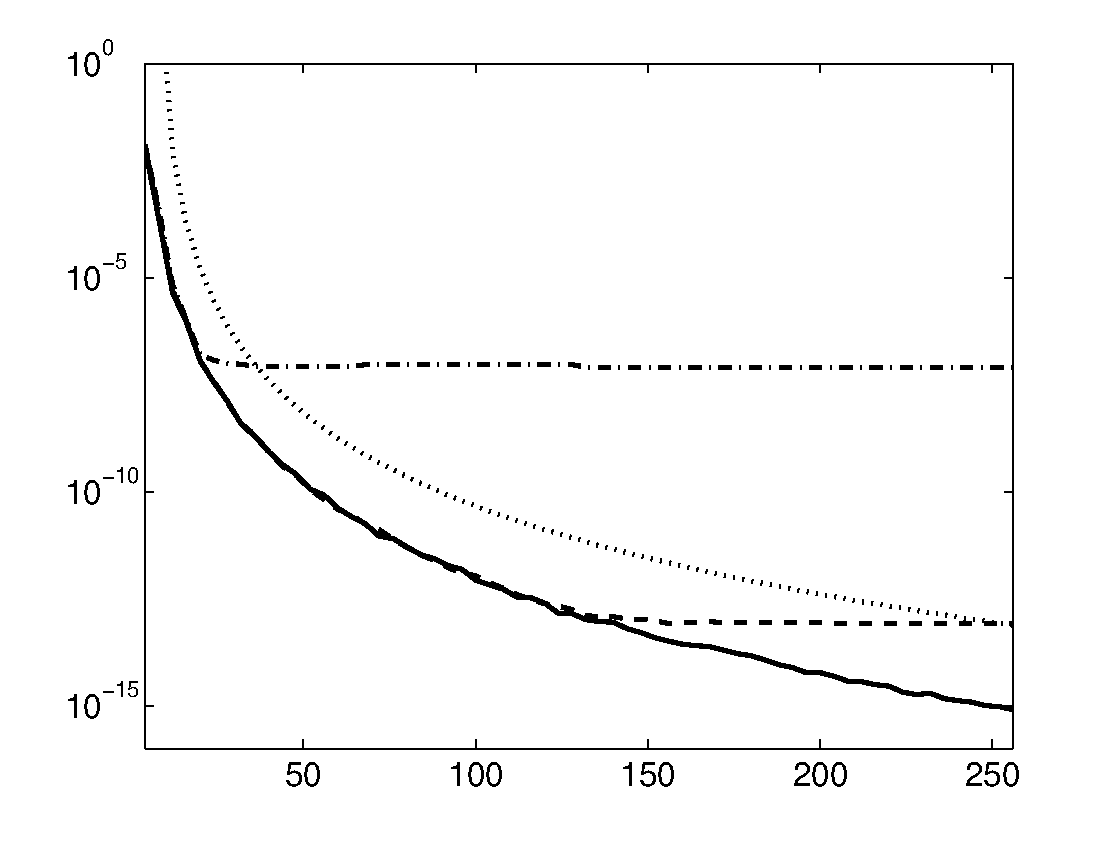
\includegraphics[width=0.45\textwidth]{images/locsupp_test}}\hfill
  \subfigure[The Gaussian kernel $G_{\sigma}$ for $\sigma=250$.]
  {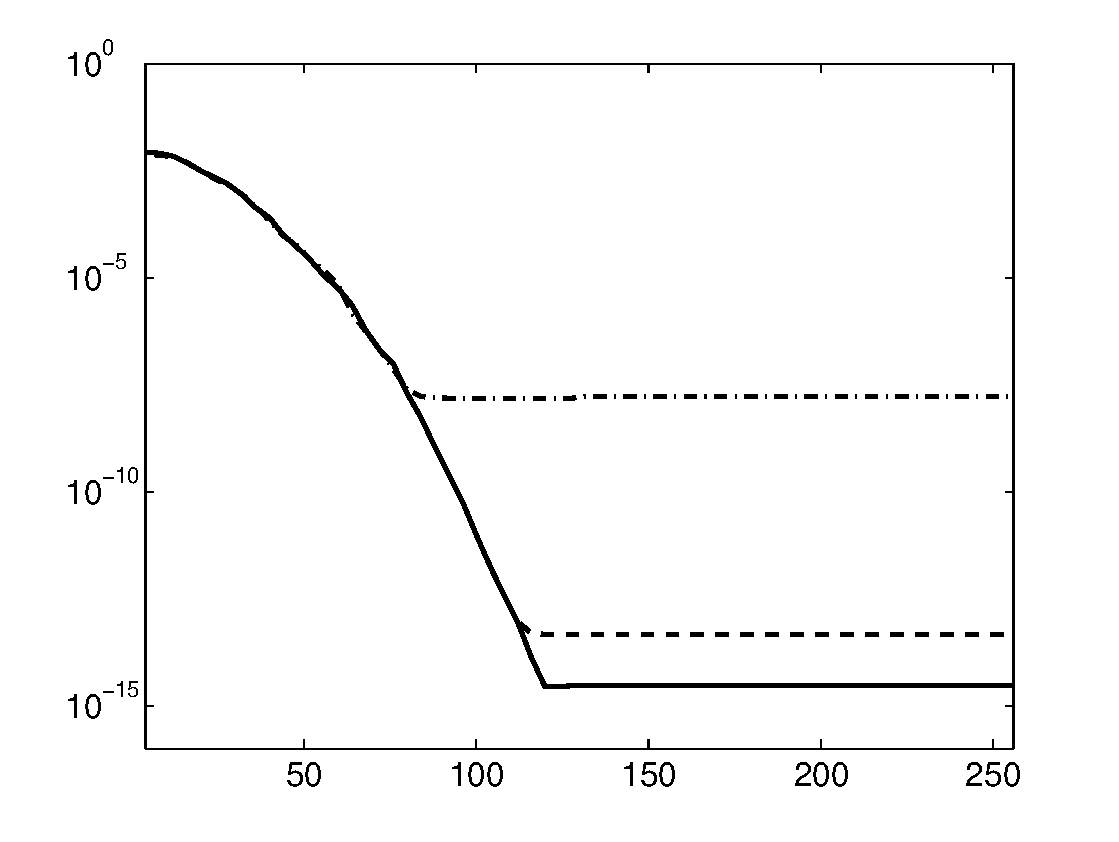
\includegraphics[width=0.45\textwidth]{images/gaussian_test}}
  \caption{The error $E_{\infty}$ for $k = 4,8,\ldots,256$ and $L = D = 1000$: 
  Fast summation with NDSFT (solid), fast summation with NFSFT, 
  cut-off parameter $m = 3$ (dash-dot), fast summation with NFSFT, cut-off 
  parameter $m = 6$ (dashed), error estimate for 
  $E_{\infty}$ (dotted).}
  \label{fig:error}
\end{figure}

\begin{figure}[tb]
  \centering
  {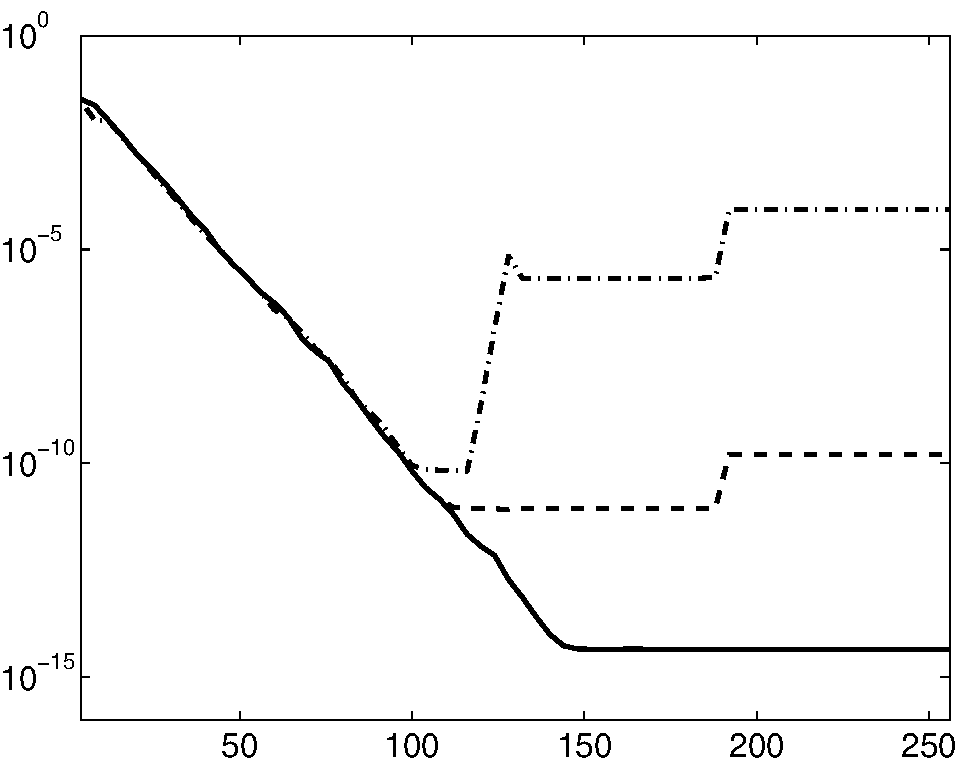
\includegraphics[width=0.45\textwidth]{images/threshold_test}}\hfill
  \subfigure[$\lambda=2.0$]
  {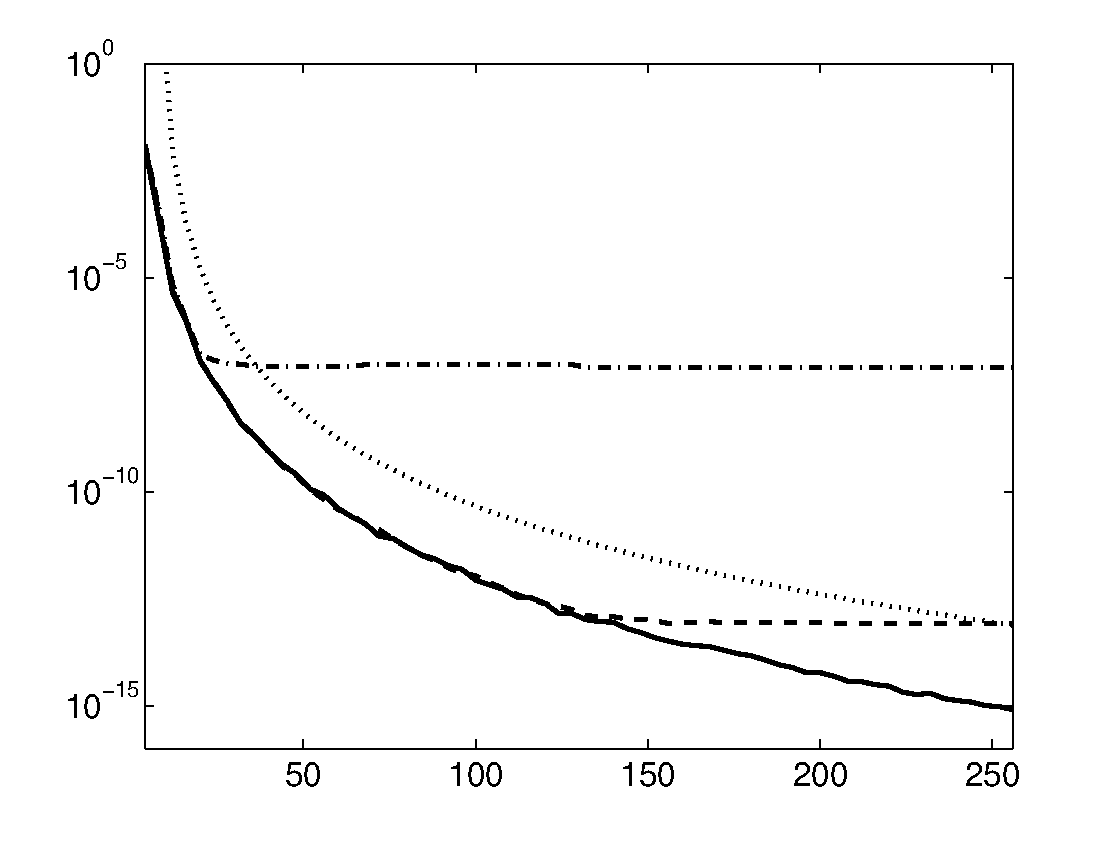
\includegraphics[width=0.45\textwidth]{images/locsupp_test}}
  \caption{To be written...}
  \label{Figure:PoissonTest}
\end{figure}

\begin{figure}[tb]
  \centering
  {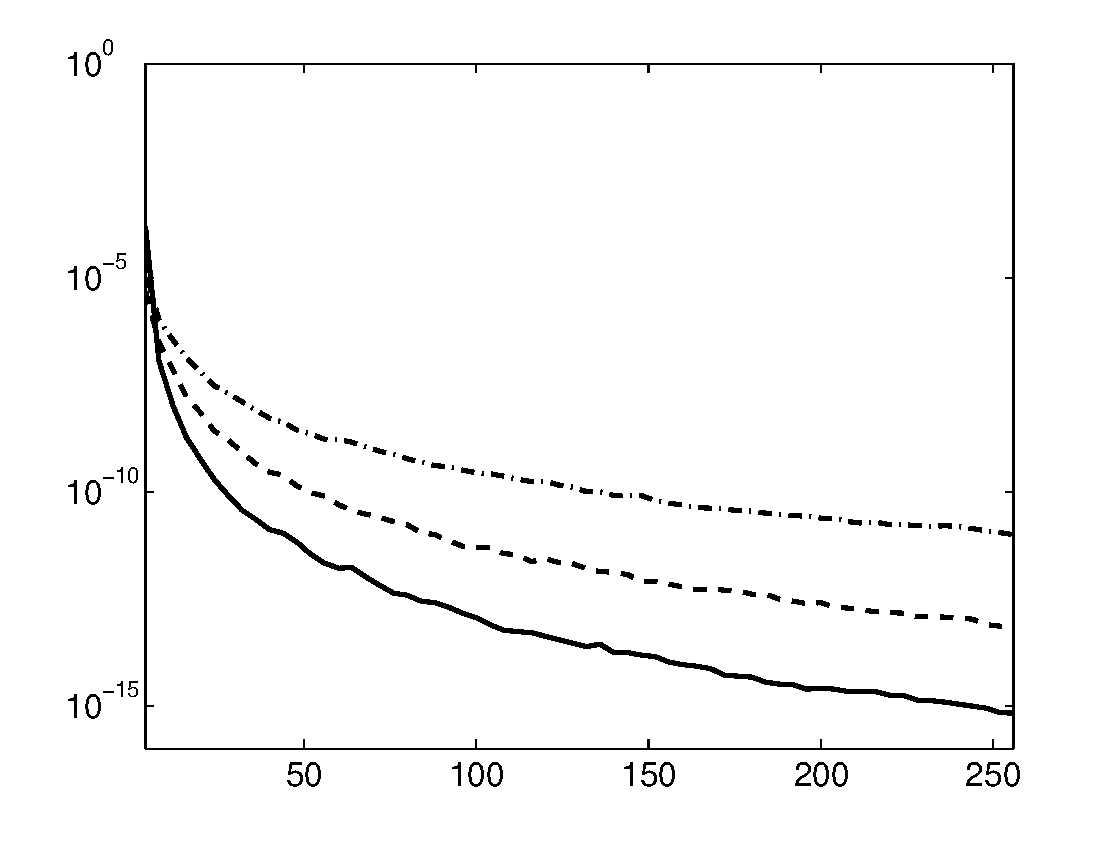
\includegraphics[width=0.45\textwidth]{images/locsupp_lambda_test}}\hfill
  \subfigure[$\lambda=2.0$]
  {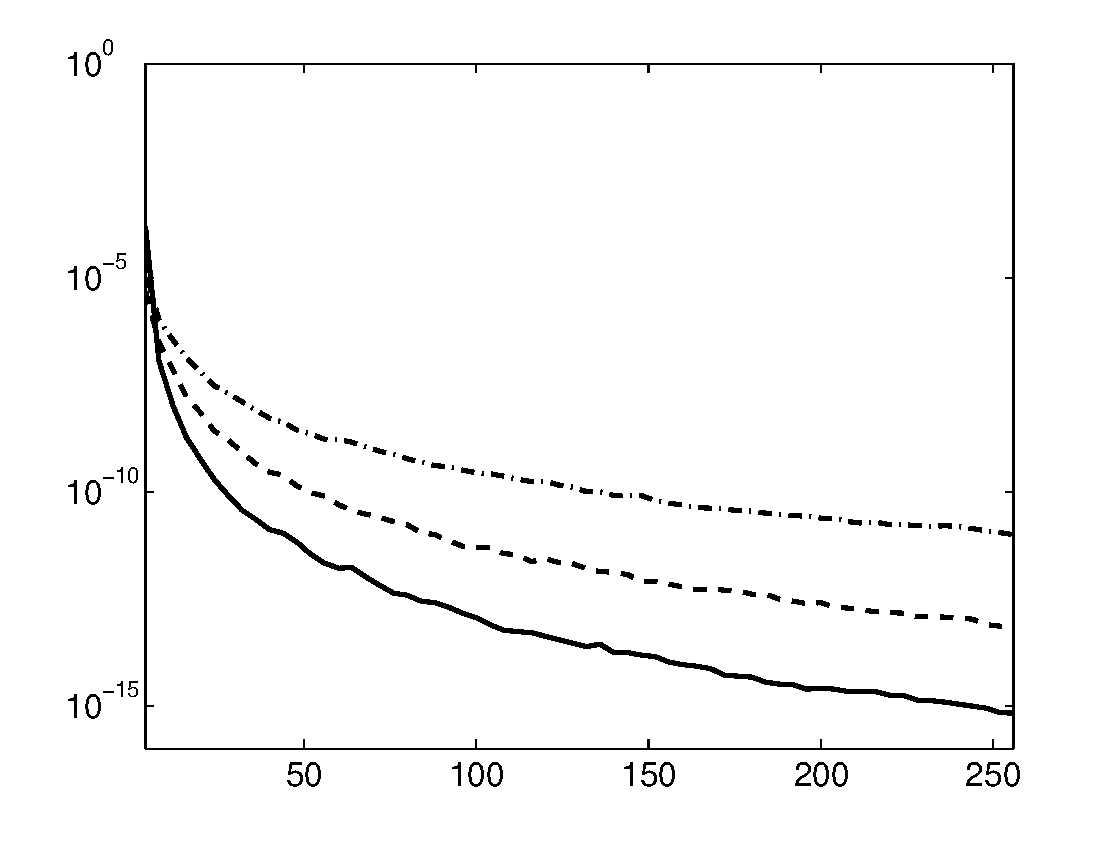
\includegraphics[width=0.45\textwidth]{images/locsupp_lambda_test}}
  \caption{To be written...}
  \label{Figure:PoissonTest}
\end{figure}

Finally, we compare the computation time of the straightforward summation, the
straightforward summation with the precomputed matrix, the fast summation
algorithm with NDSFT, and the fast summation algorithm with NFSFT for
increasing $D=L$. 
The CPU time required by the four algorithms is shown in Table
\ref{tab:TimeSpace}. 
As expected, the fast NDSFT and NFSFT summation algorithms outperform the 
straightforward algorithms, yielding an ${\cal O}(D)$ complexity in both 
variants, but with the NFSFT--version considerably faster.

\begin{table}[ht!]
  \begin{center}
    \begin{tabular}{r|r|r|r|r|r|r}
    $L$ & $D$ & direct alg. & with precomp. & FS, NDSFT & FS, NFSFT & error $E_{\infty}$\\\hline
        64 &     64 & 1.0E-03 & -- & 1.1E-01 & 6.1E-01 & 7.7E-14\\
       128 &    128 & 7.0E-03 & -- & 2.3E-01 & 6.1E-01 & 6.5E-14\\
       256 &    256 & 2.5E-02 & -- & 4.6E-01 & 6.1E-01 & 4.1E-14\\
       512 &    512 & 1.0E-01 & -- & 9.1E-01 & 6.2E-01 & 2.8E-14\\
      1024 &   1024 & 4.0E-01 & -- & 1.8E+00 & 6.5E-01 & 3.6E-14\\
      2048 &   2048 & 1.6E+00 & -- & 3.6E+00 & 6.6E-01 & 1.8E-14\\
      4096 &   4096 & 6.4E+00 & -- & 7.3E+00 & 7.2E-01 & 1.3E-14\\
      8192 &   8192 & 2.6E+01 & -- & 1.5E+01 & 8.2E-01 & 6.7E-15\\
     16384 &  16384 & 1.0E+02 & -- & 2.9E+01 & 1.0E+00 & 5.5E-15\\
     32768 &  32768 & 4.1E+02 & -- & 5.8E+01 & 1.5E+00 & 4.0E-15\\
     65536 &  65536 & 1.7E+03 & -- & 1.2E+02 & 2.3E+00 & 2.9E-15\\
    131072 & 131072 & 6.6E+03 & -- & 2.3E+02 & 4.0E+00 & 2.4E-15\\
    262144 & 262144 & 2.6E+04 & -- & 4.7E+02 & 7.5E+00 & 1.9E-15\\
    524288 & 524288 & -- & -- & 9.4E+02 & 1.4E+01 & --\\
    1048576 & 1048576 & -- & -- & 1.9E+03 & 2.8E+01 & --\\
    2097152 & 2097152 & -- & -- & 3.8E+03 & 5.6E+01 & --.\\
    \end{tabular}
  \end{center}
  \caption{CPU-Time and error $E_{\infty}$ for the fast summation algorithm.
    Note that we used accumulated measurements in case of small times and the
    times/error (*) are not displayed due to the large response time or the 
    limited size of memory.}
  \label{tab:TimeSpace}
\end{table}


%--------------------------------------------------------------------------
\section{Conclusions}
%--------------------------------------------------------------------------

We have presented a fast algorithm for the computation of sums of type
\eqref{Applications:KernelSum} in ${\cal O} (D +L)$ arithmetic operations.
We have proved error estimates concerning the dependence of the computational
speed on the desired accuracy and the parameters of particular interesting
kernels.
The software for this algorithm including all described tests is available
within the NFFT package \cite[{\tt ./example/fastsumS2}]{kupo02C}. // Can be
obtained from the authors?????

%-----------------------------------------------------------------------------
\bibliographystyle{abbrv}
\bibliography{../references}
\end{document}
